\chapter{Elektrotechnik}
\section{Grundgrößen}

\begin{boxleft}\bla{Elementarladung}
\end{boxleft}\begin{boxrightshaded}
\begin{align*}
e\approx 1,6\cdot 10^{-19}C
\end{align*}
\end{boxrightshaded}

\begin{boxleft}\bla{ele. Ladung}
\end{boxleft}\begin{boxrightshaded}
\begin{align*}
\left[Q\right]&=1C=1As\\
Q&=n\cdot e
\end{align*}
\end{boxrightshaded}

\begin{boxleft}\bla{ele. Strom}
\end{boxleft}\begin{boxrightshaded}
\begin{align*}
\left[I\right]&=1A\\
i(t)&=\frac{\diff Q}{\diff t}
\end{align*}
\end{boxrightshaded}

\begin{boxleft}\bla{ele. Stromdichte}
\end{boxleft}\begin{boxrightshaded}
\begin{align*}
\left[J\right]&=1\frac{A}{mm^2}\\
\vec{J}&=\frac{I}{\vec{A}}
\end{align*}
\end{boxrightshaded}

\begin{boxleft}\bla{ele. Potenzial}
\end{boxleft}\begin{boxrightshaded}
\begin{align*}
\left[\varphi\right]&=1V=1\frac{Nm}{As}=1\frac{kgm^2}{As^3}\\
\varphi&=\frac{W}{Q}
\end{align*}
\end{boxrightshaded}

\begin{boxleft}\bla{ele. Spannung}
\end{boxleft}\begin{boxrightshaded}
\begin{align*}
\left[U\right]&=1V\\
U_{AB}&=\varphi_a-\varphi_b
\end{align*}
\end{boxrightshaded}

\begin{boxleft}\bla{ele. Widerstand}
\end{boxleft}\begin{boxrightshaded}
\begin{align*}
\left[R\right]&=1\Omega=1\frac{V}{A}\\
R&=\frac{U}{I}\\
&=\rho\frac{l}{A}=\frac{1}{\kappa}\frac{l}{A}
\end{align*}
\end{boxrightshaded}

\begin{boxleft}\bla{ele. Leitwert}
\end{boxleft}\begin{boxrightshaded}
\begin{align*}
\left[G\right]&=1S=1\frac{A}{V}\\
G&=\frac{I}{U}\\
&=\frac{1}{R}\\
&=\kappa\frac{A}{l}=\frac{1}{\rho}\frac{A}{l}
\end{align*}
\end{boxrightshaded}

\begin{boxleft}\bla{Temperaturabhängigkeit von Widerstand}
\end{boxleft}\begin{boxrightshaded}
\begin{align*}
R_2=R_1\cdot\left(1+\alpha\left(\vartheta_2-\vartheta_1\right)+\beta\left(\vartheta_2-\vartheta_1\right)^2\right)
\end{align*}
\end{boxrightshaded}

\section{Lineare Quellen}
\begin{boxleft}\bla{Lineare Spanungsquelle}
\end{boxleft}\begin{boxrightshaded}
\begin{align*}
U&=U_q-R_i\cdot I\\
I_K&=\frac{U_q}{R_i}
\end{align*}
\end{boxrightshaded}

\begin{boxleft}\bla{Lineare Stromquelle}
\end{boxleft}\begin{boxrightshaded}
\begin{align*}
I&=I_q-\frac{U}{R_i}\\
U_l&=I_q\cdot R_i
\end{align*}
\end{boxrightshaded}

\section{Kirchhoffsche Gesetze}


\begin{boxleft}\bla{Knotenpunktsatz}
\end{boxleft}\begin{boxrightshaded}
\begin{align*}
\sum_{i=1}^n I_i=0
\end{align*}
\end{boxrightshaded}

\begin{boxleft}\bla{Maschensatz}
\end{boxleft}\begin{boxrightshaded}
\begin{align*}
\sum_{i=1}^n U_i=0
\end{align*}
\end{boxrightshaded}

\section{Wechselspannung}

\begin{boxleft}\bla{Gleichanteil}
\end{boxleft}\begin{boxrightshaded}
\begin{align*}
\bar{u}&=\frac{1}{T}\int_t^{t+T}u(t)\diff t\\
\bar{i}&=\frac{1}{T}\int_t^{t+T}i(t)\diff t
\end{align*}
\end{boxrightshaded}

\begin{boxleft}\bla{Gleichrichtwert}
\end{boxleft}\begin{boxrightshaded}
\begin{align*}
\left|\bar{u}\right|&=\frac{1}{T}\int_t^{t+T}\left|u(t)\right|\diff t\\
\left|\bar{i}\right|&=\frac{1}{T}\int_t^{t+T}\left|i(t)\right|\diff t
\end{align*}
\end{boxrightshaded}

\begin{boxleft}\bla{Effektivwert}
\end{boxleft}\begin{boxrightshaded}
\begin{align*}
u_{eff}&=U=\sqrt{\frac{1}{T}\int_t^{t+T}\left(u(t)\right)^2\diff t}\\
i_{eff}&=I=\sqrt{\frac{1}{T}\int_t^{t+T}\left(i(t)\right)^2\diff t}
\end{align*}
\end{boxrightshaded}

\begin{boxleft}\bla{Formfaktor}
\end{boxleft}\begin{boxrightshaded}
\begin{align*}
F&=\frac{u_{eff}}{\left|\bar{u}\right|}\\
F&=\frac{\pi}{2\cdot\sqrt{2}}&&\text{Sinus}
\end{align*}
\end{boxrightshaded}

\begin{boxleft}\bla{Scheitelfaktor}
\end{boxleft}\begin{boxrightshaded}
\begin{align*}
\sigma&=\frac{\hat{u}}{u_{eff}}\\
\sigma&=\sqrt{2} && \text{Sinus}
\end{align*}
\end{boxrightshaded}


\section{Sinusspannung}

\begin{boxleft}\bla{Sinusschwingung}
\des[\radian\per\second]{\omega}{Kreisfrequenz}\\
\des[\radian]{\varphi}{Phasenverschiebung}\\
\des[\volt]{\hat{u}}{Spitzenwert der Spannung}
\end{boxleft}\begin{boxrightshaded}
\begin{align*}
u(t)&=\hat{u}\sin{\left(\omega t+\varphi_u\right)}\\
i(t)&=\hat{i}\sin{\left(\omega t+\varphi_i\right)}\\
\omega&=\frac{\varphi_u}{t}=2\pi f =2\pi\frac{1}{T}\\
t_u&=-\frac{\varphi_u}{\omega}
\end{align*}
\end{boxrightshaded}

\begin{boxleft}\bla{Addition zweier Schwingungen}
\end{boxleft}\begin{boxrightshaded}
\begin{align*}
u_1(t)&=\hat{u}_1\sin{\left(\omega t+\varphi_{u1}\right)}\\
u_2(t)&=\hat{u}_2\sin{\left(\omega t+\varphi_{u2}\right)}\\
\hat{u}_{12}&=\sqrt{\hat{u}_1^2+\hat{u}_2^2+2\hat{u}_1\hat{u}_2\cos\left(\varphi_{u1}-\varphi_{u2}\right)}\\
\varphi_{u12}&=\arctan\left(\frac{\hat{u}_1\sin{\varphi_{u1}}+\hat{u}_2\sin{\varphi_{u2}}}{\hat{u}_1\cos{\varphi_{u1}}+\hat{u}_2\cos{\varphi_{u2}}}\right)\\
\text{Nenner}&<0\Rightarrow\varphi_{u12}+\pi
\end{align*}
\end{boxrightshaded}

\begin{boxleft}\bla{Komplexezeiger}
\end{boxleft}\begin{boxrightshaded}
\begin{align*}
u(t)&=\hat{u}_1\sin{\left(\omega t+\varphi_{u}\right)}\\
\underline{u}(t)&=\hat{u}\left(\cos{\left(\omega t+\varphi_{u}\right)}+j\sin{\left(\omega t+\varphi_{u}\right)}\right)\\
\underline{u}(t)&=\hat{u}e^{j\left(\omega t+\varphi_{u}\right)}
\end{align*}
\end{boxrightshaded}

\begin{boxleft}\bla{Widerstand}
\end{boxleft}\begin{boxrightshaded}
\begin{align*}
\underline{u}&=R\underline{i}\\
\underline{i}&=\frac{1}{R}\underline{u}\\
\underline{Z}&=R\\
\underline{Y}&=\frac{1}{R}\\
P&=RI^2\\
Q&=0\\
\lambda&=\cos\varphi=0
\end{align*}
\end{boxrightshaded}

\begin{boxleft}\bla{Induktivität}
\end{boxleft}\begin{boxrightshaded}
\begin{align*}
\underline{u}&=L\frac{\diff\underline{i}}{\diff t}\\
\underline{i}&=\frac{1}{L}\int\underline{u}\diff t\\
\underline{Z}&=\frac{\underline{u}}{\underline{i}}=j\omega L=\omega L e^{j\frac{\pi}{2}}\\
\underline{Y}&=\frac{\underline{i}}{\underline{u}}=\frac{1}{j\omega L}=\frac{1}{\omega L} e^{-j\frac{\pi}{2}}\\
P&=0\\
Q&=\frac{1}{\omega L}U^2\\
Q&=\omega L I^2\\
\lambda&=\cos\varphi=1
\end{align*}
\end{boxrightshaded}

\begin{boxleft}\bla{Kapazität}
\end{boxleft}\begin{boxrightshaded}
\begin{align*}
\underline{u}&=\frac{1}{C}\int\underline{i}\diff t\\
\underline{u}&=C\frac{\diff\underline{i}}{\diff t}\\
\underline{Z}&=\frac{\underline{u}}{\underline{i}}=\frac{1}{j\omega C}=\frac{1}{\omega C} e^{-j\frac{\pi}{2}}\\
\underline{Y}&=\frac{\underline{i}}{\underline{u}}=j\omega C=\omega C e^{j\frac{\pi}{2}}\\
Q&=-\omega C U^2\\
Q&=-\frac{1}{\omega C}I^2\\
\lambda&=\cos\varphi=1
\end{align*}
\end{boxrightshaded}

\subsection{Widerstand}

\begin{boxleft}\bla{Impedanz}
\des[\ohm]{Z}{Impedanz}\\
\des[\ohm]{R}{Wirkwiderstand}\\
\des[\ohm]{X}{Blindwiderstand}
\end{boxleft}\begin{boxrightshaded}
\begin{align*}
\underline{Z}&=\operatorname{Re}\{\underline{Z}\}+j\operatorname{Im}\{\underline{Z}\}=R+jX=Ze^{j\varphi}\\
\underline{Z}&=\sqrt{R^2+X^2}e^{j\arctan\frac{X}{R}}\\
\varphi&=\varphi_u-\varphi_i\\
R&=Z\cdot\cos \varphi\\
X&=Z\cdot\sin \varphi\\
X&=\omega L&L=&\frac{X}{\omega}\\
X&=-\frac{1}{\omega C}&C=&-\frac{1}{\omega X}
\end{align*}
\end{boxrightshaded}

\begin{boxleft}\bla{Admitanz}
\des[\siemens]{Y}{Admitanz}\\
\des[\siemens]{G}{Wirkleitwert(Konduktanz)}\\
\des[\siemens]{B}{Blindleitwert(Suszeptanz)}\\
\end{boxleft}\begin{boxrightshaded}
\begin{align*}
\underline{Y}&=\operatorname{Re}\{\underline{Y}\}+j\operatorname{Im}\{\underline{Y}\}=G+jB=Ye^{j\gamma}\\
\underline{Y}&=\sqrt{G^2+B^2}e^{j\arctan\frac{B}{G}}\\
\gamma&=\varphi_u-\varphi_i\\
G&=Y\cdot\cos \gamma\\
B&=Y\cdot\sin \gamma\\
B&=-\frac{1}{\omega L}&L=&-\frac{1}{\omega B}\\
B&=\omega C&C=&\frac{B}{\omega}
\end{align*}
\end{boxrightshaded}


\section{Leistung}

\begin{boxleft}\bla{Momentanleistung}
\des[\watt]{P}{Leistung}\\
\end{boxleft}\begin{boxrightshaded}
\begin{align*}
P&=u(t)\cdot i(t)
\end{align*}
\end{boxrightshaded}

\begin{boxleft}\bla{Mittlere Leistung}
\end{boxleft}\begin{boxrightshaded}
\begin{align*}
P&=\frac{1}{T}\int_0^T u(t)\cdot i(t)\diff t \\
P&=UI\cdot \cos{\left(\varphi_u-\varphi_i\right)}\\
P&=\operatorname{Re}\{S\}
\end{align*}
\end{boxrightshaded}

\begin{boxleft}\bla{Blindleistung}
\des[var]{S}{Scheinleistung}
\end{boxleft}\begin{boxrightshaded}
\begin{align*}
Q&=UI\cdot\sin{\left(\varphi_u-\varphi_i\right)}\\
Q&=\operatorname{Im}\{S\}
\end{align*}
\end{boxrightshaded}

\begin{boxleft}\bla{Scheinleistung}
\des[var]{S}{Scheinleistung}
\end{boxleft}\begin{boxrightshaded}
\begin{align*}
\underline{S}&=\underline{Z}I^2\\
\underline{S}&=RI^2+jXI^2\\
\underline{S}&=P+jQ\\
S&=\left|\underline{S}\right|\\
S&=U\cdot I
\end{align*}
\end{boxrightshaded}

\begin{boxleft}\bla{Leistungsfaktor}
\end{boxleft}\begin{boxrightshaded}
\begin{align*}
\lambda&=\frac{P}{S}\\
\lambda&=\cos{\left(\varphi_u-\varphi_i\right)} && \text{Sinus}
\end{align*}
\end{boxrightshaded}
\newpage
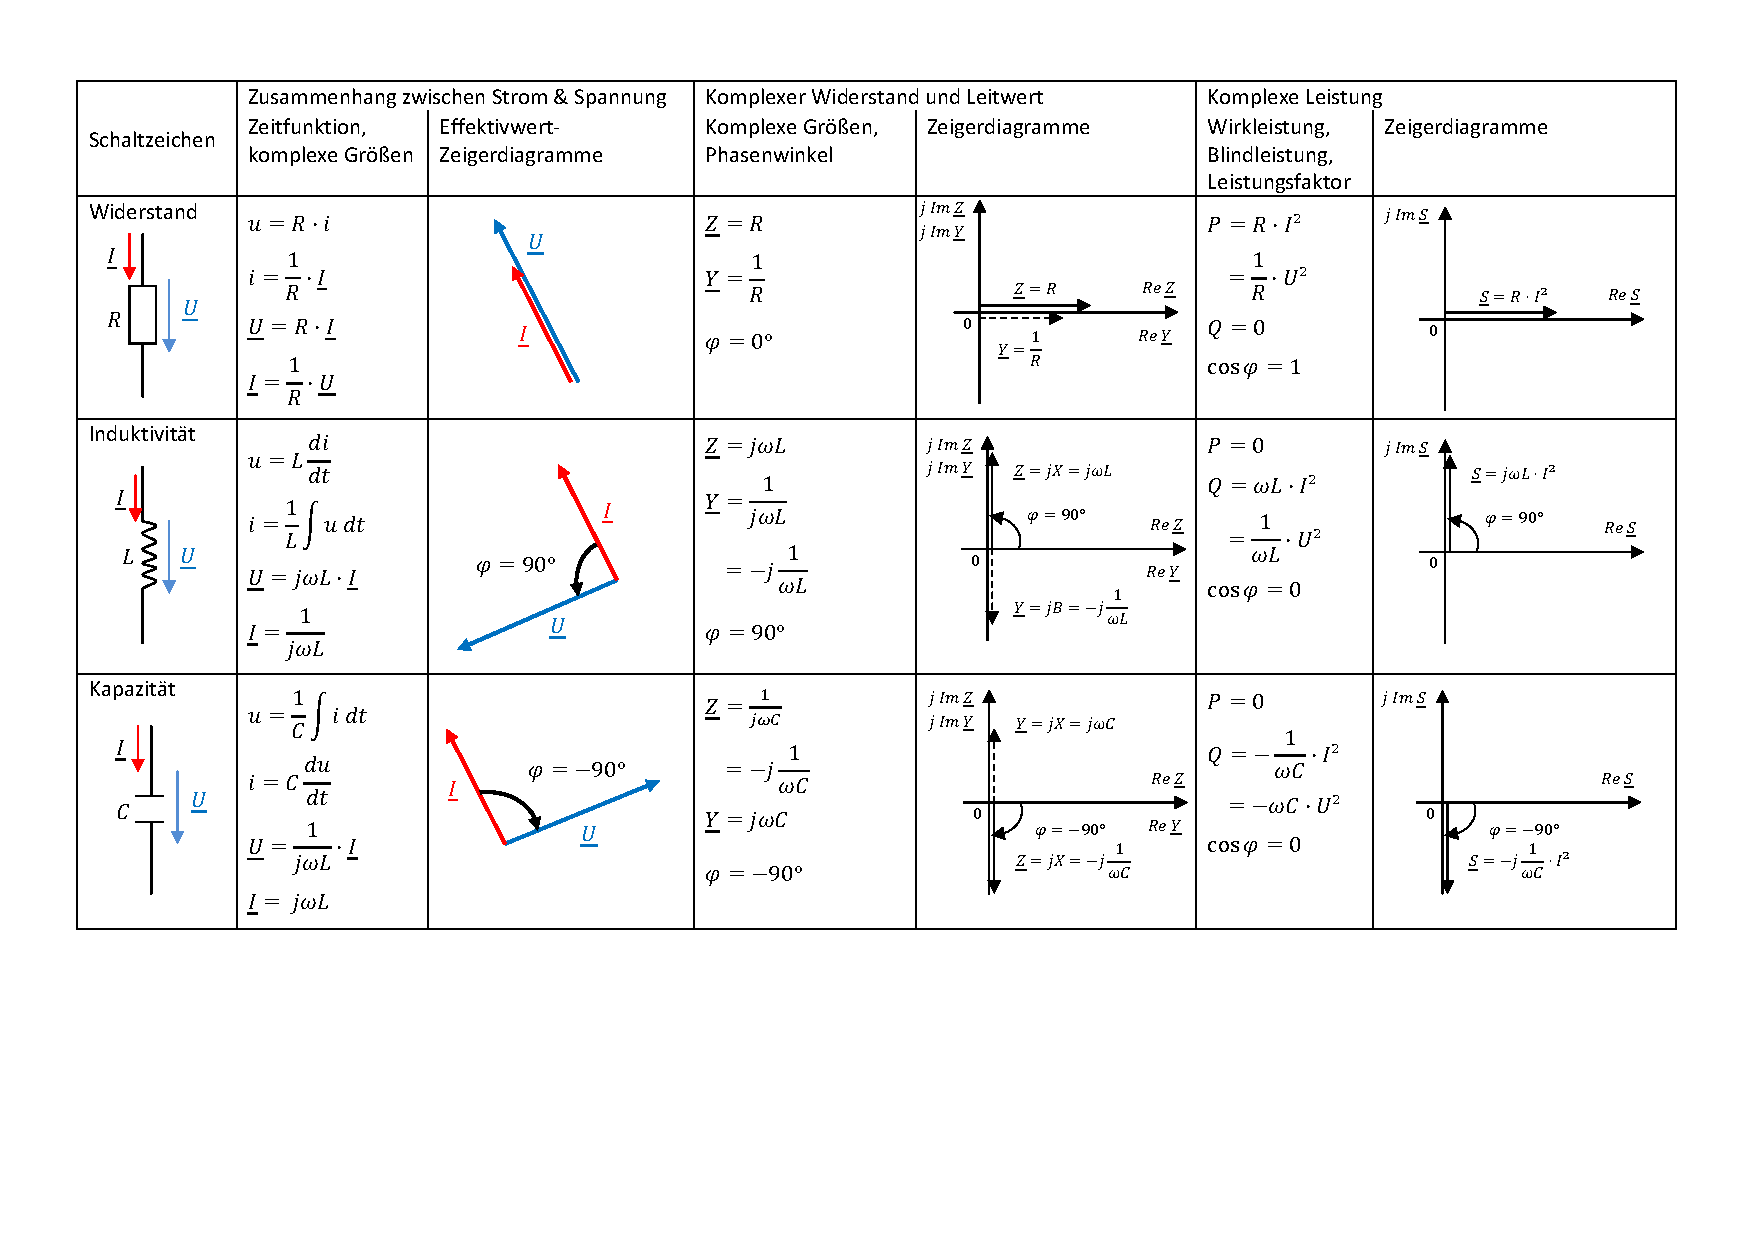
\includepdf[fitpaper=true]{elektro/pdf/diagram1.pdf}
\newpage

